\documentclass[letterpaper,12pt]{article}
\usepackage{array}
\usepackage{threeparttable}
\usepackage{geometry}
\geometry{letterpaper,tmargin=1in,bmargin=1in,lmargin=1.25in,rmargin=1.25in}
\usepackage{fancyhdr,lastpage}
\pagestyle{fancy}
\lhead{}
\chead{}
\rhead{}
\lfoot{}
\cfoot{}
\rfoot{\footnotesize\textsl{Page \thepage\ of \pageref{LastPage}}}
\renewcommand\headrulewidth{0pt}
\renewcommand\footrulewidth{0pt}
\usepackage[format=hang,font=normalsize,labelfont=bf]{caption}
\usepackage{listings}
\lstset{frame=single,
  language=Python,
  showstringspaces=false,
  columns=flexible,
  basicstyle={\small\ttfamily},
  numbers=none,
  breaklines=true,
  breakatwhitespace=true
  tabsize=3
}
\usepackage{amsmath}
\usepackage{amssymb}
\usepackage{amsthm}
\usepackage{harvard}
\usepackage{setspace}
\usepackage{float,color}
\usepackage[pdftex]{graphicx}
\usepackage{hyperref}
\hypersetup{colorlinks,linkcolor=red,urlcolor=blue}
\theoremstyle{definition}
\newtheorem{theorem}{Theorem}
\newtheorem{acknowledgement}[theorem]{Acknowledgement}
\newtheorem{algorithm}[theorem]{Algorithm}
\newtheorem{axiom}[theorem]{Axiom}
\newtheorem{case}[theorem]{Case}
\newtheorem{claim}[theorem]{Claim}
\newtheorem{conclusion}[theorem]{Conclusion}
\newtheorem{condition}[theorem]{Condition}
\newtheorem{conjecture}[theorem]{Conjecture}
\newtheorem{corollary}[theorem]{Corollary}
\newtheorem{criterion}[theorem]{Criterion}
\newtheorem{definition}[theorem]{Definition}
\newtheorem{derivation}{Derivation} % Number derivations on their own
\newtheorem{example}[theorem]{Example}
\newtheorem{exercise}[theorem]{Exercise}
\newtheorem{lemma}[theorem]{Lemma}
\newtheorem{notation}[theorem]{Notation}
\newtheorem{problem}[theorem]{Problem}
\newtheorem{proposition}{Proposition} % Number propositions on their own
\newtheorem{remark}[theorem]{Remark}
\newtheorem{solution}[theorem]{Solution}
\newtheorem{summary}[theorem]{Summary}
%\numberwithin{equation}{section}
\bibliographystyle{aer}
\newcommand\ve{\varepsilon}
\newcommand\boldline{\arrayrulewidth{1pt}\hline}


\begin{document}

\begin{flushleft}
  \textbf{\large{Problem Set \#2}} \\
  MACS 30100, Dr. Evans \\
  Bobae Kang
\end{flushleft}

\vspace{5mm}

\begin{enumerate}
\item \textbf{Some income data, lognormal distribution, and hypothesis testing.}
\begin{enumerate}
\item Plot a histogram of percentages of the income.txt data with 30 bins. Make sure that the bins are weighted such that the height of each bin represents the percent of the income observations in that bin. In other words, all the bin heights should sum to 1. Make sure your plot has correct x-axis and y-axis labels as well as a plot title.
\par
\begin{figure}[H]\centering\captionsetup{width=4.0in}
   \fbox{\resizebox{4.0in}{3.0in}{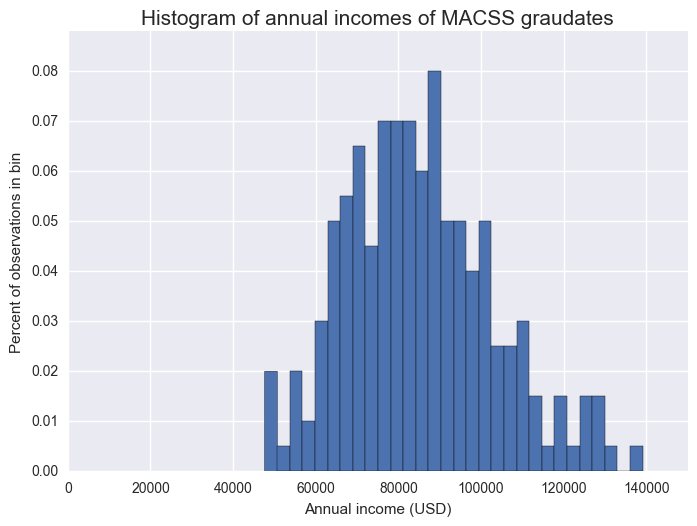
\includegraphics{./images/fig_1a.png}}}
\end{figure}
\par\bigskip

\item Plot the lognormal PDF $f(x|\mu = 9.0, \sigma = 0.3)$ for 0 $\leq x \leq$ 150,000. What is the value of the log likelihood value for this parameterization of the distribution and given this data?
\par
\begin{figure}[H]\centering\captionsetup{width=4.0in}
  \fbox{\resizebox{4.0in}{3.0in}{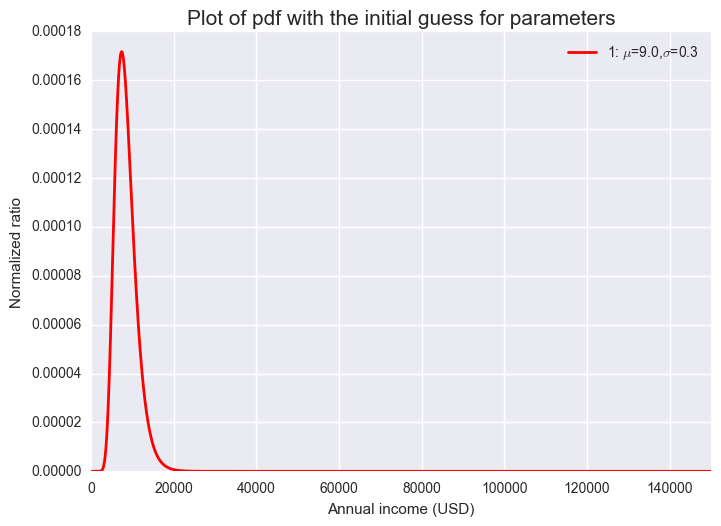
\includegraphics{./images/fig_1b.png}}}
\end{figure}
\par
Log-likelihood value = -8298.63695601
\par\bigskip

\item Estimate the parameters of the lognormal distribution by maximum likelihood and plot its PDF against the PDF from part (b) and the histogram from part (a). Plot the estimated PDF for 0 $\leq x \leq$ 150,000. Report the ML estimates for $\mu$ and $\sigma$, the value of the likelihood function, and the variance-covariance matrix.
\par
\begin{figure}[H]\centering\captionsetup{width=4.0in}
  \fbox{\resizebox{4.0in}{3.0in}{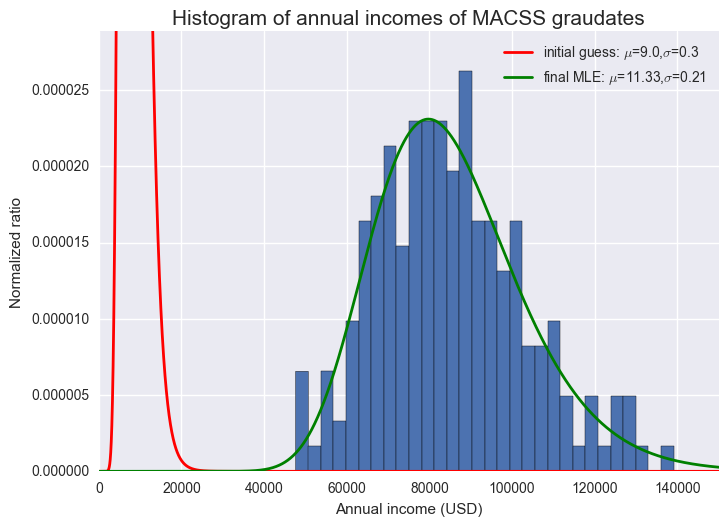
\includegraphics{./images/fig_1c.png}}}
\end{figure}
\par
MLE estimate for $\mu$ = 11.331440374 \par
MLE estimate for $\sigma$ = 0.211674587081 \par
Log-likelihood value = -2239.5347439980096 \par
VCV =  [[  2.47898671e-04   2.46830454e-06] \par
\hspace{12mm} [  2.46830454e-06   1.12322196e-04]]
\par\bigskip

\item Perform a likelihood ratio test to determine the probability that the data in `incomes.txt` came from the distribution in part (b).
\par\bigskip
$\chi^2$ of $H_{0}$ with 2 degrees of freedom p-value =  0.0
\par\bigskip

\item With your estimated distribution of incomes for Chicago MACSS students from part (c), you now have a model for what your own income might look like when you graduate. Using that estimated model from part (c), What is the probability that you will earn more than $\$$100,000? What is the probability that you will earn less than $\$$75,000?
\par\bigskip
The probability that you will earn more than \$100,000 is: 19.56\%
\par
The probability that you will earn less than \$75,000 is: 30.79\%
\par\bigskip
\end{enumerate}

\item \textbf{ Linear regression and MLE}
\begin {enumerate}
\item Estimate the parameters of the model $(\beta_{0}, \beta_{1}, \beta_{2}, \beta_{3}, \sigma^2)$ by maximum likelihood using the fact that each error term $\varepsilon_i$ is distributed normally $N(0, \sigma^2)$. Report your estimates, the value of the log likelihood function, and the estimated variance covariance matrix of the estimates.
\par\bigskip
MLE estimate for $\beta_{0}$ = 0.251644293661  \par
MLE estimate for $\beta_{1}$ = 0.0129334154112 \par
MLE estimate for $\beta_{2}$ = 0.400501865882 \par
MLE estimate for $\beta_{3}$= -0.00999168487451 \par
MLE estimate for $\sigma^2$ = 9.10892518541e-06 \par
Log-likelihood value = 876.865053329\par
VCV = [[ 1.  0.  0.  0.  0.] \par
\hspace{12mm}   [ 0.  1.  0.  0.  0.] \par
\hspace{12mm}   [ 0.  0.  1.  0.  0.] \par
\hspace{12mm}   [ 0.  0.  0.  1.  0.] \par
\hspace{12mm}   [ 0.  0.  0.  0.  1.]]
\par\bigskip

\item Use a likelihood ratio test to determine the probability that $\beta_0$ = 1.0, $\sigma^2$ = 0.01 and $\beta_1, \beta_2, \beta_3$ = 0. That is, what is the likelihood that age, number of children, and average winter temperature have no effect on the number of sick days?
\par\bigskip
The $\chi^2$ of $H_0$: age, number of childeren, and average winter temperature have no effect on the number of sick days, with 5 degrees of freedom, is: 0.

\end {enumerate}
\end {enumerate}

\end{document}
